\documentclass[conference]{IEEEtran}
\IEEEoverridecommandlockouts
\usepackage{cite,amsmath,amssymb,graphicx,booktabs,url}
\usepackage[hidelinks]{hyperref}
\def\BibTeX{{\rm B\kern-.05em{\sc i\kern-.025em b}\kern-.08em T\kern-.1667em\lower.7ex\hbox{E}\kern-.125emX}}
%% auto-generated; do not edit
\newcommand{\ModelMedRel}{11.3\%}
\newcommand{\ModelMeanRel}{16.1\%}
\newcommand{\NGraphs}{120}
\newcommand{\PhaseAControl}{0.489}
\newcommand{\DelayBaseline}{8.88}
\newcommand{\BudgetFifty}{5.6}
\newcommand{\NFitsFifty}{5}
\newcommand{\BudgetSecond}{113}
\newcommand{\NFitsSecond}{7}
\newcommand{\NDelayMethods}{11}
\newcommand{\GTShortPath}{0.600}
\newcommand{\GTMaxWeight}{0.531}
\newcommand{\GTRandom}{0.490}
\newcommand{\NControls}{3}
\newcommand{\ModelMAE}{2.22}
\newcommand{\KoneOracleFid}{+1.21}
\newcommand{\KoneOracleSE}{0.75}
\newcommand{\KoneShortPathFid}{-5.39}
\newcommand{\KoneShortPathSE}{1.24}
\newcommand{\KoneSaliencyFid}{-5.98}
\newcommand{\KoneSaliencySE}{1.02}
\newcommand{\KoneNBigger}{6}
\newcommand{\KoneNOther}{9}
\newcommand{\KoneWorstFid}{-7.30}
\newcommand{\KoneWorstSE}{1.73}
\newcommand{\KoneWorstName}{Deconvolution}
\newcommand{\KoneOracleZ}{1.6}
\newcommand{\SeedN}{3}
\newcommand{\SeedQualities}{11.3\%, 12.7\% and 17.1\%}
\newcommand{\SeedNMethods}{8}
\newcommand{\SeedNWord}{three}
\newcommand{\NTransfer}{9}
\newcommand{\NTransferWord}{nine}
\newcommand{\TransferBAMin}{0.80}
\newcommand{\NSat}{7}
\newcommand{\NSatWord}{Seven}
\newcommand{\SatBASpan}{0.009}
\newcommand{\SatRoutMin}{0.59}
\newcommand{\SatRoutMax}{0.90}
\newcommand{\SatRoutSpan}{0.306}
\newcommand{\SeedNMethodsWord}{eight}
\newcommand{\SeedGTSpread}{0.015}
\newcommand{\SeedFidSpread}{2.17}
\newcommand{\SeedFlipName}{InputXGradient}
\newcommand{\SeedFlipFid}{-0.03}
\newcommand{\SeedFlipHalf}{3.48}
\newcommand{\SeedWorstGTName}{PGExplainer}
\newcommand{\SeedWorstGTMean}{0.485}
\newcommand{\SeedWorstGTHalf}{0.147}
\newcommand{\SeedCtrlGTHalf}{0.0000}
\newcommand{\SeedCtrlFidHalf}{1.02}
\newcommand{\AggrMinMean}{11.3\%}
\newcommand{\AggrMinOnly}{18.8\%}
\newcommand{\AggrMeanOnly}{27.2\%}
\newcommand{\DecoyZeroMaxWeightAUC}{0.994}
\newcommand{\DecoyZeroMaxWeightRec}{0.858}
\newcommand{\DecoyZeroBestName}{Deconvolution}
\newcommand{\DecoyZeroBestAUC}{0.805}
\newcommand{\DecoyThreeMaxWeightAUC}{0.483}
\newcommand{\DecoyThreeDeconvAUC}{0.874}
\newcommand{\MagThreeDeconv}{0.897}
\newcommand{\MagThreeShortPath}{0.787}
\newcommand{\MagThreeModel}{9.5\%}
\newcommand{\MagTwentyFourDeconv}{0.856}
\newcommand{\MagTwentyFourShortPath}{0.583}
\newcommand{\MagTwentyFourModel}{17.2\%}
\newcommand{\MagTwelveDeconv}{0.875}


\begin{document}

\title{Ground-Truth Evaluation of Graph Neural Network\\Explainers for Network Routing}

% TODO(author): name spelling and the three affiliation lines below are the
% only remaining placeholders in this file. Verify the name as you publish it.
\author{\IEEEauthorblockN{Mohamed Ali Ben Azzouna}
\IEEEauthorblockA{\textit{Department} \\ \textit{Institution} \\ City, Country \\
mohamedali.benazzouna@outlook.com}}

\maketitle

\begin{abstract}
Explainable AI for software-defined routing is evaluated almost exclusively
using \emph{fidelity}, which measures how much a model's prediction changes
when the edges identified as important by an explanation are removed. This
reliance reflects a practical limitation: operational routing data provide no
ground-truth explanations. We construct such a reference using 229 real
topologies. For each sample, we introduce a bottleneck link and verify its
effect on shortest-path cost; we also add decoy links drawn from the same
weight distribution but placed off the active route. Thus, identifying the
true bottleneck requires reasoning about topology and traffic flow rather than
simply ranking link weights. We evaluate eleven explainers against this ground
truth, ten of which we first validate on the standard BA-Shapes benchmark. Our results yield two main findings. First, BA-Shapes performance
does not predict routing performance: GNNExplainer and PGExplainer decline
from approximately $0.99$ to $0.59$ and $0.63$, respectively, approaching the
performance of a control that does not use the model. By contrast, gradient-
and Shapley-sampling methods achieve scores of $0.77$--$0.91$. LIME and KernelSHAP, widely used in applied work, are the
weakest methods on the standard benchmark and remain in the lower half on
routing, where the learned-mask methods rank lowest.
Second, fidelity and ground truth lead to different assessments of explainer
quality. Fidelity also fails to distinguish published methods from controls
that do not use the model, even as the predictive model becomes more accurate,
and its values are unstable across independent training runs where
ground-truth recovery is not.
Moreover, the commonly recommended soft-masking remedy is ineffective for
the minimum-aggregation architecture used here. Finally, we measure explanation latency against published
control-plane budgets: \NFitsFifty{} of \NDelayMethods{} methods fit a
$50$\,ms protection-switching interval, and the three perturbation methods
miss a sub-second one by orders of magnitude.
\end{abstract}

\begin{IEEEkeywords}
explainable AI, graph neural networks, network routing, fidelity, evaluation
\end{IEEEkeywords}

\section{Introduction}
Graph neural networks (GNNs) are increasingly used for data-driven network
modelling and routing. Their limited interpretability has consequently
motivated growing interest in explanation methods. In the explainable
software-defined routing literature, explanations are commonly evaluated
using \emph{fidelity}: edges identified as important are removed, and the
resulting change in the model's prediction is treated as evidence that the
explanation has captured the information on which the model relies.

Fidelity remains common because operational routing data do not record
\emph{why} a path is slow, leaving no reference explanation to evaluate
against. But it is an indirect proxy whose validity is widely questioned:
removing edges can move an input outside the model's training distribution, so
the resulting change may reflect the perturbation rather than the explanation's
quality. This has been examined for images, text and time series, with
mitigations proposed for those modalities. Whether it arises for graph
regression in routing is untested.

This work addresses that gap by providing a reference against which
explanations can be assessed. Our contributions are:

\begin{itemize}
  \item \textbf{A routing task with verified explanation ground truth}
  (Section~\ref{sec:data}). Planting ground truth is established practice; the
  \emph{decoy} construction this domain needs is not. A bottleneck is planted
  in real topologies and verified per sample to change the shortest-path cost;
  heavy decoys from its own weight range neutralise the model-free rules that
  otherwise top the leaderboard.
  \item \textbf{A transfer study} (Section~\ref{sec:transfer}). Ten explainers
  are first verified against published figures on BA-Shapes, then measured on
  routing under the identical metric.
  \item \textbf{Evidence that fidelity is unreliable here}
  (Sections~\ref{sec:fidelity}--\ref{sec:soft}): it scores a known-correct
  explanation below a model-free one, and the remedy prescribed for its known
  weakness does not apply to the aggregation that makes the task learnable.
  \item \textbf{Delay measurements} (Section~\ref{sec:delay}) placing each
  method against published control-plane timing budgets.
\end{itemize}

\section{Related Work}
\label{sec:related}
\textbf{Explaining GNNs.} Post-hoc explainers for graph models fall into three
families. Learned-mask methods optimise a soft edge mask per instance, as in
GNNExplainer~\cite{ying2019gnnexplainer}, or amortise that optimisation into a
generator trained once, as in PGExplainer~\cite{luo2020pgexplainer} and
GraphMask~\cite{schlichtkrull2021graphmask}. Backpropagation methods attribute
the output to the input in one or a few passes; integrated
gradients~\cite{sundararajan2017ig} is the most widely used. Perturbation
methods fit a local surrogate or estimate Shapley values by repeated
occlusion, as in LIME~\cite{ribeiro2016lime} and SHAP~\cite{lundberg2017shap}; surveys
organise these families and their metrics~\cite{li2022survey}. Our line-up
spans all three, which matters because
they behave very differently once moved out of the benchmark setting into
this one.

\textbf{Evaluating explanations without ground truth.} Because reference
explanations are rarely available, the field evaluates with fidelity: delete
what the explanation marks as important and measure the change in the
prediction. The weakness of this proxy is well documented. Zheng
\emph{et~al.}~\cite{zheng2024robustfidelity} give an information-theoretic
account showing that $\mathrm{Fid}^{+}$, $\mathrm{Fid}^{-}$ and
$\mathrm{Fid}_{\Delta}$ are distorted by the distribution shift that subgraph
removal induces, and propose robust variants. F-Fidelity~\cite{zheng2025ffidelity}
attacks the same problem by fine-tuning the model under explanation-agnostic
random masking so that perturbed inputs stay in distribution. Both are
developed and evaluated
for images, text and time series, and for classification. Whether their
conclusions hold for graph regression is untested, and we find one of their
remedies inapplicable to the architecture this task requires
(Section~\ref{sec:soft}).

\textbf{Ground-truth explanation datasets.} The alternative is to construct
data whose explanations are known by design. BA-Shapes~\cite{ying2019gnnexplainer}
established the pattern for graphs: plant motifs and treat their edges as the
reference. Mir\'o-Nicolau \emph{et~al.}~\cite{mironicolau2023fidelity} take this
furthest for fidelity specifically, building synthetic image datasets with
reference explanations and comparing thirteen methods against them; they report
that backpropagation methods are more reliable than sensitivity-analysis
methods such as LIME and SHAP. Our results agree in direction while differing in
domain, model class and task: we observe the same ordering on graphs under
regression, where perturbation methods are weakest. We are not aware of a
ground-truth explanation benchmark for routing, which is what
Section~\ref{sec:data} supplies.

\textbf{GNNs for networking.} Graph models are standard for network
performance prediction, with RouteNet-Fermi~\cite{ferriol2023routenetfermi}
representative of per-flow delay regression, and for routing control as policy
or value approximators~\cite{almasan2022drlgnn}. The applied
explainable-routing literature has correspondingly adopted post-hoc
explainers, predominantly LIME and SHAP, evaluated by fidelity because
operational data carry no reference explanation. That combination --- the two
families we find weakest, assessed with the metric we find unreliable ---
motivates this study.

\section{A Routing Task With Explanation Ground Truth}
\label{sec:data}
\subsection{Topologies and labels}
We use 229 real topologies (203 from the Internet Topology
Zoo~\cite{knight2011topologyzoo} and 26 from SNDlib~\cite{orlowski2010sndlib}),
retaining graphs with 20--50 nodes. Link propagation delay is derived from
great-circle length. Each sample draws a source--destination pair and is
labelled with the Dijkstra shortest-path cost, transformed by $\log(1+x)$ and
standardised. Splits are partitioned \textbf{by topology name}: over a few dozen distinct
graphs a sample-level split would let the model memorise each topology, and
every reported number would be in-distribution.

\subsection{Planted bottlenecks and decoys}
In each evaluation graph one link is raised to $12\times$ the graph's median
link delay. A plant is accepted only if it changes the Dijkstra cost by at
least $10\%$, verified per sample rather than assumed, so the ground-truth
edge is causally relevant by construction. Raising uses
$\max(\text{existing}, \text{planted})$, since plain assignment can
\emph{lower} a link on real topologies whose delays span orders of magnitude.

Without decoys the task is solved by a two-line rule that never consults the
model: sort links by weight.
Regenerating this dataset without decoys and retraining, that heuristic
reaches \DecoyZeroMaxWeightAUC{} AUC and \DecoyZeroMaxWeightRec{} Recall@1, above
every explainer (best: \DecoyZeroBestName{} at \DecoyZeroBestAUC), so the task would
be measuring whether a method can read \texttt{edge\_attr}. We therefore plant up to nine additional heavy links drawn from the
\emph{same} weight distribution but placed off the active route. The route is
recomputed \emph{after} the bottleneck is planted, and decoys are sampled
without replacement from the edges absent from that post-planting optimal
path, capped at a quarter of the graph's links. Raising the weight of an edge
that is not on the shortest path cannot change that path's cost, so decoys are
provably label-preserving; this is asserted per sample. Three decoys already
suppress the weight heuristic to \DecoyThreeMaxWeightAUC{} while Deconvolution
holds \DecoyThreeDeconvAUC; nine reduce a lucky guess among the heavy links to
about one in ten. Link weight alone therefore cannot identify which heavy link constrains the flow: given ten of them, which matters for \emph{this} path?

\subsection{The explained model}
\label{sec:model}
Shortest-path cost is defined by a minimum over candidate paths, making it poorly suited to models that rely on averaging. The natural baseline is a graph
attention network~\cite{velickovic2018gat}, which the attention-based
explainers require and which we retain for the delay comparison of
Section~\ref{sec:delay}. But it aggregates by softmax-weighted averaging, and
stacking such layers does not represent a minimum. Following the observation that path-finding
algorithms require selecting one optimal neighbour per
step~\cite{velickovic2020neuralexec}, we instead use
GENConv~\cite{li2020deepergcn}, whose message is
$\mathrm{relu}(x_j + W_e e_{ij})$, with \texttt{min} aggregation included:
the layer then computes $\min_j (x_j + w_{ij})$, which is the Bellman--Ford
relaxation step. We set the depth to 10 iterations, covering the measured 90th-percentile path length of nine hops. Aggregation is
\texttt{min+mean}, because \texttt{min} alone passes gradient only to the
arg-min neighbour: on identical data and hyperparameters, median relative
error is \AggrMinMean{} for \texttt{min+mean}, \AggrMinOnly{} for \texttt{min}
and \AggrMeanOnly{} for \texttt{mean}. The readout concatenates mean pooling with the source and
destination node embeddings. On held-out topologies, the model achieves a median relative error of \ModelMedRel{} and a mean relative error of \ModelMeanRel{}. A constant predictor scores $70.9\%$. Rerunning Dijkstra on the model's own inputs reproduces every label exactly, so the task carries no irreducible label noise.

\section{Experimental Setup}
\label{sec:setup}
\subsection{Explainers}
We evaluate eleven methods spanning the commonly used explainer families.
Nine attribute to an \emph{edge mask}: GNNExplainer and PGExplainer (learned
masks); Integrated Gradients, Input$\times$Gradient, Deconvolution and Guided
Backpropagation (backpropagation); and LIME, KernelSHAP and Shapley value
sampling (perturbation). All are driven through published
implementations~\cite{fey2019pyg,kokhlikyan2020captum}.

Two further variants attribute to the \emph{link weight} $\mathbf{e}$ rather
than to a mask, computing $\partial f/\partial \mathbf{e}$ directly: we denote
these IG (edge-weight) and Saliency (edge-weight). They answer a different
question --- how sensitive is the predicted cost to this link's delay, rather
than to its presence --- which is the quantity a routing operator can act on.
Because they require edge features, they cannot be run on BA-Shapes, which has
none; they therefore appear in the routing results only, and the BA-Shapes
validation covers the remaining ten methods.

All learned-mask methods are fitted on the routing training split, not
transferred from BA-Shapes: GNNExplainer optimises a mask per explained graph,
and PGExplainer's generator is trained on 400 routing training graphs. Any
difference between the two domains therefore reflects the task, not a reused
model. \NControls{} controls are reported in every
table, none of which consults the model: \textsc{MaxWeight} scores a link by
its own weight, \textsc{ShortestPath} scores the links carrying the flow, and
\textsc{Random} is the floor. The first two correspond to the two kinds of
prior information a planted bottleneck leaks. Weight is controlled for by the
decoy construction; path membership is not, because a decoy placed on the
active route would change the label, so \textsc{ShortestPath} measures what
that residual leak is worth. It is not privileged information: the mask is
Dijkstra over the model's own inputs. If a method cannot outperform scoring rules that do not use the model, it provides no evidence that its explanations reflect the model's behaviour.

Perturbation budgets require clarification because they are defined differently across methods: LIME and KernelSHAP draw $n$ perturbations in total, whereas Shapley sampling draws $n$ perturbations \emph{per feature}. We use $n=400$ for the first two,
measured to be at LIME's plateau, and $n=25$ for Shapley sampling.

\subsection{Metrics}
\textbf{Ground-truth recovery.} We evaluate explanations as binary edge classifiers, using the planted link as the positive class, and report ROC-AUC. Scores are first computed per directed arc and then aggregated to physical links by taking the maximum across the two directions. We use attribution magnitude because a large negative attribution can still indicate an important edge.

\textbf{Fidelity.} We use the score-based variant appropriate to regression,
signed and unnormalised, in milliseconds of predicted path cost:
$\mathrm{Fid}^{+} = \frac{1}{N}\sum_i [f(G_i) - f(G_i \setminus e_i)]$ and
$\mathrm{Fid}^{-} = \frac{1}{N}\sum_i [f(G_i) - f(e_i)]$.
We report the two separately and do not combine them into the
characterisation score of~\cite{li2022survey}, the harmonic mean of
$\mathrm{Fid}^{+}$ and $1-\mathrm{Fid}^{-}$, because that combination assumes
$\mathrm{Fid}^{-}\!\in\![0,1]$, which a regression output in milliseconds
violates.

Model quality is reported as median relative error,
$\mathrm{median}_i\,|\hat{y}_i - y_i| / \max(|y_i|, \epsilon)$ over held-out
graphs, with $\hat{y}$ and $y$ inverse-transformed to milliseconds. The median
is used because path costs span three orders of magnitude.

\textbf{Delay.} Per-explanation wall-clock time against one batch-1 forward
pass, measured round-robin so that drift affects all methods equally, and
reported as bands rather than a ranking.

\subsection{Harness validation}
We first validate every method on BA-Shapes, where planted house motifs
provide explanation ground truth.
Table~\ref{tab:transfer}'s \emph{Pub.} and BA-Shapes columns show that the
harness reproduces or exceeds the published figures --- GNNExplainer $0.991$
against $0.925$~\cite{ying2019gnnexplainer}, PGExplainer $1.000$ against
$0.963$~\cite{luo2020pgexplainer}, random control \PhaseAControl{} --- so a
weak routing result cannot be attributed to it.

\section{BA-Shapes Performance Does Not Predict Routing Performance}
\label{sec:transfer}
\begin{table}[t]
\centering
\small
\caption{Explanation quality under one metric in two domains: explanation as binary edge classification against ground truth. BA-Shapes anchors the harness against published figures; routing is the planted bottleneck against the off-path decoys, which share its weight distribution and so neutralise any advantage from reading edge features. Chance is 0.5.}
\label{tab:transfer}
\begin{tabular}{lrrrr}
\toprule
Explainer & Pub. & BA-Shapes & Routing & $\Delta$ \\
\midrule
IntegratedGradients & -- & 0.995 & 0.866 & $-0.128$ \\
ShapleyValueSampling & -- & 0.994 & 0.896 & $-0.098$ \\
Deconvolution & -- & 0.996 & 0.875 & $-0.122$ \\
InputXGradient & -- & 0.995 & 0.864 & $-0.131$ \\
GuidedBackprop & -- & 0.996 & 0.773 & $-0.223$ \\
KernelSHAP & -- & 0.803 & 0.750 & $-0.053$ \\
LIME & -- & 0.928 & 0.712 & $-0.216$ \\
\midrule
PGExplainer & 0.963 & 1.000 & 0.625 & $-0.375$ \\
GNNExplainer & 0.925 & 0.991 & 0.590 & $-0.401$ \\
\midrule
MaxWeight (control) & -- & -- & 0.531 & -- \\
Random (control) & -- & 0.478 & 0.490 & $+0.012$ \\
\bottomrule
\end{tabular}
\end{table}


\begin{figure}[t]
\centering
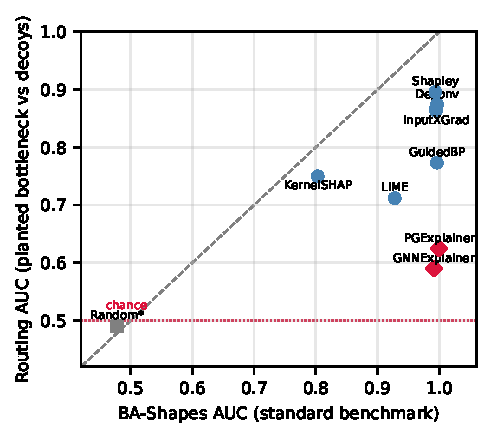
\includegraphics[width=\columnwidth]{figures/fig_transfer.pdf}
\caption{Explanation quality on the standard benchmark (horizontal) against
the routing task (vertical), same metric. Points on the dashed diagonal would
transfer perfectly. The learned-mask methods (diamonds) fall to just above the
chance line; controls are squares.}
\label{fig:transfer}
\end{figure}

Table~\ref{tab:transfer} and Fig.~\ref{fig:transfer} compare both domains
under one metric, so differences reflect the methods and not the measurement.

First, all \NTransfer{} methods score between \TransferBAMin{} and $1.00$ on
BA-Shapes, against a control at $0.478$.

Second, they are not equivalent on routing. Integrated Gradients ($0.866$),
Shapley sampling ($0.896$) and Deconvolution ($0.875$) retain most of their
accuracy, whereas \textbf{GNNExplainer falls to $0.590$ and PGExplainer to
$0.625$} --- against \NControls{} model-free controls at \GTShortPath,
\GTMaxWeight{} and \GTRandom. Neither is distinguishable from the strongest of
them, a model-free rule scoring the links that carry the flow ($|z|<1$ both). Both learn a
mask by optimising a sufficiency objective on the model's own output, and that
objective is satisfiable on this task without locating the planted link.
PGExplainer is also the least stable method across training runs
(Section~\ref{sec:fidelity}).

Third, and of practical relevance here, LIME ($0.712$) and KernelSHAP
($0.750$) are the weakest non-control methods on routing and already weakest
on BA-Shapes ($0.928$ and $0.803$). KernelSHAP's deficit is not a sampling
artefact: raising its budget from 25 to 650 draws moves its BA-Shapes AUC from
$0.831$ to $0.812$. These are the two methods applied explainable-SDN work
relies on most.

The $\Delta$ column is not a robustness measure: a method starting at $0.996$
has more room to fall than one at $0.803$, so small drops at the bottom of the
benchmark column are a floor effect.
The more informative comparison is among methods whose benchmark scores are
near saturation. \NSatWord{} of the \NTransferWord{} methods sit at or above
$0.99$ on BA-Shapes, a span of \SatBASpan; \emph{within that group} routing
AUC spans \SatRoutSpan, from \SatRoutMin{} to \SatRoutMax. A near-ceiling score on the standard
benchmark is therefore necessary evidence that an explainer is correctly
implemented --- which is why we establish it first --- but it cannot
discriminate among methods that all saturate it, and it does not transfer into
a prediction about a new domain. These results motivate domain-specific ground
truth; they do not diminish the value of standard benchmarks.

\section{Fidelity Disagrees With Ground Truth}
\label{sec:fidelity}
\begin{table}[t]
\centering
\small
\caption{The two metrics disagree. Ground-truth AUC is recovery of the planted bottleneck against the decoys; Fid$^+$ is the signed change in predicted path cost when the explanation is removed, with the standard error of its mean. The last column reports whether Fid$^+$ is distinguishable from \emph{all three} controls at $|z|>2$. Nine of eleven methods recover the bottleneck above $0.70$; three are separable under fidelity.}
\label{tab:contradiction}
\begin{tabular}{lrr@{\,$\pm$\,}lc}
\toprule
Explainer & GT AUC & \multicolumn{2}{c}{Fid$^+$ (ms)} & $\ne$ controls \\
\midrule
IG (ours, edge-weight) & 0.914 & -2.77 & 2.08 & -- \\
ShapleyValueSampling & 0.896 & +8.04 & 1.98 & \checkmark \\
Saliency (ours, edge-weight) & 0.875 & -14.01 & 2.41 & \checkmark \\
Deconvolution & 0.875 & -5.84 & 2.48 & -- \\
IntegratedGradients & 0.866 & -0.84 & 2.31 & -- \\
InputXGradient & 0.864 & -2.83 & 2.66 & -- \\
GuidedBackprop & 0.773 & +2.03 & 2.41 & -- \\
KernelSHAP & 0.750 & +2.61 & 1.56 & -- \\
LIME & 0.712 & +8.37 & 1.66 & \checkmark \\
PGExplainer & 0.625 & -2.75 & 0.95 & -- \\
GNNExplainer & 0.590 & -3.65 & 1.14 & -- \\
\midrule
ShortestPath (control) & 0.600 & -7.39 & 2.06 & -- \\
MaxWeight (control) & 0.531 & +1.16 & 0.72 & -- \\
Random (control) & 0.490 & -2.17 & 0.75 & -- \\
\bottomrule
\end{tabular}
\end{table}


Table~\ref{tab:contradiction} places both metrics side by side for every
method. Nine of the eleven explainers recover the planted
bottleneck above $0.70$ AUC, against \NControls{} controls spanning
\GTRandom{} to \GTShortPath; under
fidelity only three are distinguishable from \emph{all} of them at $|z|>2$.
The strongest method by ground
truth, integrated gradients over link weights at $0.914$, has
$\mathrm{Fid}^{+} = -2.77 \pm 2.08$\,ms, indistinguishable from a scorer that
never consults the model. LIME, at $0.712$ the third-weakest non-control method at locating the
bottleneck, is one of the three that fidelity does separate: ranking by
fidelity can overlook the methods that locate it best.

\textbf{Model accuracy does not explain this disagreement.} Because fidelity relies on the model responding meaningfully to perturbations,
one objection is that the model is not accurate enough --- which predicts that
fidelity sharpens as accuracy improves. We tested two models of the same
architecture family differing only in capacity, at $15.0\%$ and $11.3\%$ median
relative error, under the identical eight mask-based methods. It did not: the
number of methods separating from the controls fell from three to one as
accuracy improved, while ground-truth recovery held at six of eight and no
method's AUC moved by more than $0.02$. A third model of a different
architecture at $20.8\%$ error behaved comparably, but used a different method
set and is not directly comparable.

\textbf{Nor does it depend on the training run.} We repeated the measurement
on \SeedNWord{} independent runs of the same configuration (\SeedQualities{}
median relative error) under the \SeedNMethodsWord{} mask-based methods. Ground-truth AUC
is stable --- median half-range \SeedGTSpread{} --- while
$\mathrm{Fid}^{+}$ is not: median half-range
\SeedFidSpread\,ms on values of a few milliseconds, and for \SeedFlipName{}
($\SeedFlipFid \pm \SeedFlipHalf$\,ms) the sign itself is undetermined. The
controls localise the cause. Their explanations are identical in every run, so
their ground-truth AUC cannot move (half-range \SeedCtrlGTHalf) --- yet their
$\mathrm{Fid}^{+}$ moves by up to \SeedCtrlFidHalf\,ms. The variance is in the
model's response to deletion, not in the explanations being compared. The one
exception under ground truth is \SeedWorstGTName{} at $\SeedWorstGTMean \pm
\SeedWorstGTHalf$, whose recovery is itself run-dependent.

The disagreement is not an artefact of the metrics measuring different
things. Recomputing fidelity at link granularity over the
top $k\!\in\!\{1,3,5\}$ links --- matching the ground-truth metric's
granularity and selection size --- does not reconcile them, and the control
failure persists at every $k$; at $k=5$ the random control's
$|\mathrm{Fid}^{+}|$ exceeds GNNExplainer's.

At $k=1$ the budget is one link, which permits a sharper question: what does
fidelity award an explanation known to be correct? An \textsc{Oracle} naming
the planted link scores $\mathrm{Fid}^{+}=\KoneOracleFid \pm
\KoneOracleSE$\,ms --- indistinguishable from zero ($|z|=\KoneOracleZ$) and
below the model's own mean absolute error of $\ModelMAE$\,ms --- at
ground-truth AUC $1.000$. \KoneNBigger{} of the \KoneNOther{} other rows move
the prediction further, including \textsc{ShortestPath} ($\KoneShortPathFid$\,ms)
and \KoneWorstName{} ($\KoneWorstFid$\,ms). Fidelity rewards deleting a link
the prediction is sensitive to; here that is not the link that sets the label.

\textbf{Sensitivity to the construction.} Regenerated at $3\times$ and
$24\times$ the bottleneck magnitude and retrained, ground-truth recovery barely
moves (Deconvolution \MagThreeDeconv, \MagTwelveDeconv, \MagTwentyFourDeconv),
so the comparison is not an artefact of that choice. The path control is
sensitive to it: at $3\times$ the planted link usually stays on the route and
\textsc{ShortestPath} rises to \MagThreeShortPath, far above both learned-mask
methods, against \GTShortPath{} at $12\times$. Path-membership leakage is a
property of a planted benchmark's configuration, not a constant.

\subsection{Why fidelity fails here}
Fidelity measures whether removing the edges selected by an explanation changes the prediction; it does not establish whether those edges cause the predicted outcome. The two come apart when a model is well fitted: as the network
learns the task it distributes its dependence over many edges, so removing a
small set perturbs it less, and the measured effect for a correct explanation
shrinks toward the noise floor. That is visible in the table as
$\mathrm{Fid}^{+}$ magnitudes of a few milliseconds sitting on standard errors
of comparable size.

Deletion is also not a neutral operation. Removing edges yields a graph unlike
any seen in training, so part of the measured change reflects the model
leaving its training distribution rather than the explanation's quality.
Section~\ref{sec:soft} shows that the remedy normally prescribed for this is
unavailable on the architecture required for the task.

Ground-truth recovery avoids these issues: it compares a ranking against a
known answer rather than depending on the model's response to perturbed
inputs, which is why its values are stable where fidelity's are not.

\section{The Soft-Masking Remedy Does Not Apply}
\label{sec:soft}
The established diagnosis for fidelity's unreliability is that hard removal
takes the input off-distribution, and the established remedy is to perturb
softly, scaling an edge's contribution toward zero rather than deleting it.
Here soft masking does not merely weaken the perturbation; it changes the
quantity measured.

Over 60 graphs with the top three links selected, hard removal yields a mean
$\mathrm{Fid}^{+}$ of $-14.73$\,ms, whereas soft-masking the \emph{same} links
toward zero yields $+9.97$\,ms. The two are \emph{anti}-correlated
($r=-0.554$) and agree on the direction of the effect in only $13\%$ of
graphs; scaling to $0.1$ rather than $0$ changes little ($+9.79$\,ms,
$r=-0.555$). This behaviour follows from the model's aggregation operation. A soft mask multiplies the
message, and GENConv's messages are strictly positive; under \texttt{min}
aggregation, scaling one toward zero makes it the minimum, so the edge being
suppressed comes to \emph{dominate} the aggregation rather than vanish from it.
Multiplicative masking expresses removal only for sum or mean aggregation.

The finding is therefore specific: \texttt{min}-like aggregation is what lets
the model learn shortest-path cost, and it is also what makes the standard
soft-masking remedy unsuitable for this architecture family. The claim concerns the fidelity
\emph{metric} only. It does \emph{not} extend to perturbation-based explainers,
which we tested directly: Shapley sampling and KernelSHAP show the smallest
transfer losses of any methods measured. We did not measure whether the distortion preserves edge \emph{ordering}
within a graph, which would be the natural reconciliation, and do not claim
it: the anti-correlation is between per-graph aggregates, not edge rankings. Why methods built on an operation that misrepresents removal
nonetheless recover the planted link remains open.

\section{Explanation Delay}
\label{sec:delay}
\begin{table}[t]
\centering
\small
\caption{One-time and per-explanation cost. Online cost is a multiple of one batch-1 forward pass. Only PGExplainer amortises: it trains a mask generator once, after which each explanation is cheap. Perturbation methods carry no training cost but pay it back many times over per explanation, since each draws hundreds of forward passes.}
\label{tab:delay}
\begin{tabular}{lrrl}
\toprule
Explainer & Offline & Online & Band \\
 & (one-time) & ($\times$ fwd) & \\
\midrule
Random (control) & -- & 0.00 & free \\
MaxWeight (control) & -- & 0.01 & free \\
Saliency (ours, edge-weight) & -- & 1.86 & cheap \\
PGExplainer & 104\,s & 3.45 & costly \\
Deconvolution & -- & 4.95 & costly \\
InputXGradient & -- & 5.03 & costly \\
GuidedBackprop & -- & 5.07 & costly \\
GNNExplainer & -- & 50.80 & offline \\
IG (ours, edge-weight) & -- & 62.83 & offline \\
IntegratedGradients & -- & 143.34 & offline \\
LIME & -- & 805.65 & offline \\
KernelSHAP & -- & 919.00 & offline \\
ShapleyValueSampling & -- & 3148.84 & offline \\
\bottomrule
\end{tabular}
\end{table}




An explanation is useful in a routing control loop only if it can be generated
within the loop's operational constraints. Table~\ref{tab:delay} separates the
two costs that matter operationally: a \emph{one-time} cost paid before the
system is deployed, and the \emph{online} cost paid for every explanation
thereafter.

Only PGExplainer incurs a one-time cost. It trains a mask generator over the
training graphs, which takes $104$\,s here, after which each explanation needs
a single forward pass through that generator. Every other method is
training-free and pays its entire cost online.

Online costs span more than three orders of magnitude, from edge saliency at
$1.9\times$ a forward pass to Shapley sampling at $3149\times$, which draws
hundreds of forward passes \emph{per edge}. The methods the applied routing
literature relies on most are therefore the least deployable inside a control
loop, by a wide margin.

PGExplainer's amortisation is real but modest: its one-time cost is repaid
against GNNExplainer after roughly $250$ explanations, and the generator must
be refitted whenever the model is, which on a changing network is a recurring
rather than a one-time cost.

One architectural caveat belongs here. Attention-based explainers read
coefficients the prediction pass has already computed and are therefore the
only methods that can be nearly free; measured on a graph attention network
they add $3\%$ to a forward pass. They do not exist on an architecture that
aggregates by minimum, so the \emph{free} band is empty for the model studied
here: the choice of architecture and the available explainers are not
independent.
We stress that these
measurements place methods in \emph{bands}; on a CPU, scheduling noise is
comparable to the gaps between neighbouring methods, so the rank within a band
should not be read as meaningful.

The ratios are hardware-specific, but they can be anchored at one end.
Carrier transport networks target a $50$\,ms protection switch~\cite{itu2018g841},
and sub-second reconvergence is the established engineering target for
link-state IGPs~\cite{francois2005subsecond}. Against the \DelayBaseline\,ms
forward pass measured here, those intervals permit $\BudgetFifty\times$ and
$\BudgetSecond\times$ a forward pass: \NFitsFifty{} of \NDelayMethods{}
methods fit inside the protection-switching budget and \NFitsSecond{} inside
the sub-second one, while the three perturbation methods miss even the looser
target by one to two orders of magnitude. What the anchor fixes is the
interval, not the hardware --- faster silicon scales every ratio down together
and leaves the ordering, and therefore which methods clear which budget,
unchanged.

\section{Limitations}
\label{sec:limits}
The \SeedNMethodsWord{} mask-based methods were measured on \SeedNWord{}
independent training runs; the three perturbation methods and every delay measurement come
from \textbf{one}. Point estimates in the tables are from the primary run, and
gaps between closely ranked methods should be read against the spreads in
Section~\ref{sec:fidelity}. The analysis
in Section~\ref{sec:fidelity} is constructed so that its conclusion does not
depend on the model's absolute accuracy. Measurements were
taken on an Intel Core i7-8550U CPU without GPU acceleration, which is why
delay is reported as bands. Labels are analytic shortest-path costs and
therefore describe propagation delay without queueing dynamics. Fidelity is
evaluated as $\mathrm{fid}^{\mathrm{prob}}$ under hard removal; a soft
perturbation that interpolates toward the mean message rather than toward zero
would avoid the pathology of Section~\ref{sec:soft}, but no existing
implementation provides one. Finally, our conclusions are limited to one architecture family and one label type; they should not be interpreted as a general characterisation of fidelity.

\section{Conclusion}
We constructed a routing task with verified explanation ground truth and showed that performance on a standard GNN explanation benchmark does not predict performance on routing: GNNExplainer and PGExplainer fall to near-chance, and
LIME and KernelSHAP --- the methods applied work relies on most --- are weakest
in both domains. Fidelity, the metric routing research uses, disagrees with that ground truth,
fails to separate published explainers from controls that never consult the
model, does not sharpen as accuracy improves, and is unstable across training
runs where ground-truth recovery is not. The remedy proposed for its known
weakness cannot be applied to the aggregation that makes routing learnable.
Where a ground truth can be constructed it should be preferred; where it
cannot, fidelity results in this domain warrant more caution than they
receive.

\bibliographystyle{IEEEtran}
\bibliography{refs}
\end{document}
